
\section{Abstract}
The learning problem for Factorial Hidden Markov Models with discrete and multi-variate latent variables remains a challenge. Inference of the latent variables required for the E-step of Expectation Minimization algorithms is usually computationally intractable. In this paper we propose a variational learning approach mimicking the Baum-Welch algorithm. By approximating the filtering distribution with a variational distribution parameterized by a recurrent neural network, the computational complexity of the learning problem as a function of the number of hidden states can be reduced to quasilinear instead of quadratic time as required by traditional algorithms such as Baum-Welch whilst making minimal independence assumptions. We evaluate the performance of the resulting algorithm, which we call Variational BOLT, in the context of unsupervised end-to-end energy disaggregation. Specifically, we conduct experiments on the publicly available REDD dataset and show competitive results when compared with a supervised inference approach and state-of-the-art results in an unsupervised setting.


\section{Introduction}
Because of its potential to discover and unlock energy saving opportunities in buildings, the problem of energy disaggregation~\cite{hart1992} has received increased interest from various academic communities. The objective of this single-channel source separation problem, also known as non-intrusive load monitoring (NILM), is to infer appliance-level power consumption information given data from only a single sensing point at the main electrical panel of a building. The observed aggregate power measured at the main panel constitutes the sum of the power of the individual appliances. Since, appliance states (e.g., {\em on}, {\em off}) can be assumed to evolve independently and the aggregate observation is dependent on the joint state of all appliances, Factorial Hidden Markov Models (FHMM)~\cite{ghahramani1997factorial} have emerged as a prominent model for the generative process of the aggregate observations. However, because latent states become conditionally dependent given the observations, exact inference of the posterior, i.e. the distribution of appliance states given the aggregate observation, is assumed to be intractable. Numerous approximate inference techniques have been proposed and employed in the past to tackle this problem. Authors in~\cite{kolter2012fhmm} introduced the one-at-a-time constraint that postulates that only a single appliance can change its state at any given time. This constraint allows for posterior inference by either posing the problem as an integer programming problem~\cite{kolter2012fhmm} or by truncating the Viterbi algorithm~\cite{lange2016efficient}. However, these approaches were focused on the decoding rather than the learning problem. On the other hand, ~\cite{jia2015fully} proposed a solution to the learning problem based on MCMC sampling but this approach seems to struggle with slow mixing of the posterior.\\
The model introduced in this paper makes use of a highly tractable auxiliary distribution that approximates the true filtering distribution. This tractable distribution is parameterized by a deep recurrent neural network, specifically stacked LSTMs~\cite{hochreiter1997long}. We build on recent results showing how neural networks in conjunction with Variational Inference can be used as a powerful tool for statistical inference~\cite{kingma2013auto}. This combination is favorable because Variational Inference allows one to pose statistical inference as a (non-linear) optimization problem and neural networks have become a dominant approach for non-linear optimization.\\
Because we assume the latent variables to be binary (i.e. a Bernoulli auxiliary distribution) we face the additional difficulty of dealing with non-conjugate discrete distributions, which pose significant challenges in the context of neural networks and variational inference \cite{kingma2013auto}. As we will show later, this problem is circumvented by directly approximating the expectation of the true filtering distribution and introducing a loss function that directly penalizes the neural network outputs for deviating from that approximation. By making use of a tractable auxiliary distribution and making minimal independence assumptions (i.e. only posterior independence of the latent variables at a single time point) computations required for the filtering distribution that are typically quadratic in the number of hidden states can be reduced to quasilinear time. This ultimately allows modeling rich temporal dependencies between latent variables whilst keeping computational costs low. Although we focus on the application of energy disaggregation in this paper, our proposed method could find applications in other fields where FHMMs with binary latent states are employed such as in certain Bioinformatics problems, e.g., \cite{stanculescu2014hierarchical,asif2011large}.\\
The decreased computational costs for inference afford our solution with the additional advantage of addressing security and privacy concerns associated with energy disaggregation solutions. In other words, disaggregation can, in principle, be carried out in real-time on cheap off-the-shelf embedded hardware located within the premises.\\
In the next section, we introduce Factorial Hidden Markov Models and explain the need for variational approximation of the filtering distribution. The section that follows shows how variational estimates of the filtering distribution can be obtained efficiently. The next section highlights the importance of modeling temporal dependencies and shows how this can be achieved by additionally modeling the difference signal of the aggregate observations. We then present experiments/results on the REDD dataset and conclusions.

\section{Factorial Hidden Markov Models and Variational Inference}

\begin{figure*}[h]
\centering
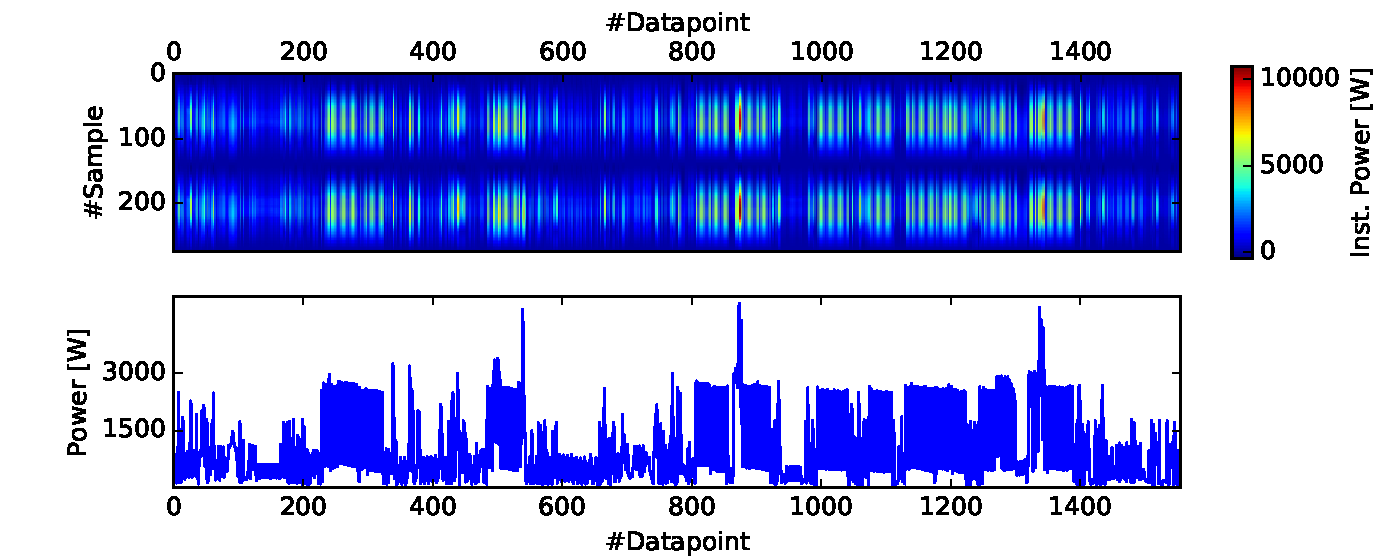
\includegraphics[width=0.95\textwidth]{varbolt/matrixX_rev.pdf}\\
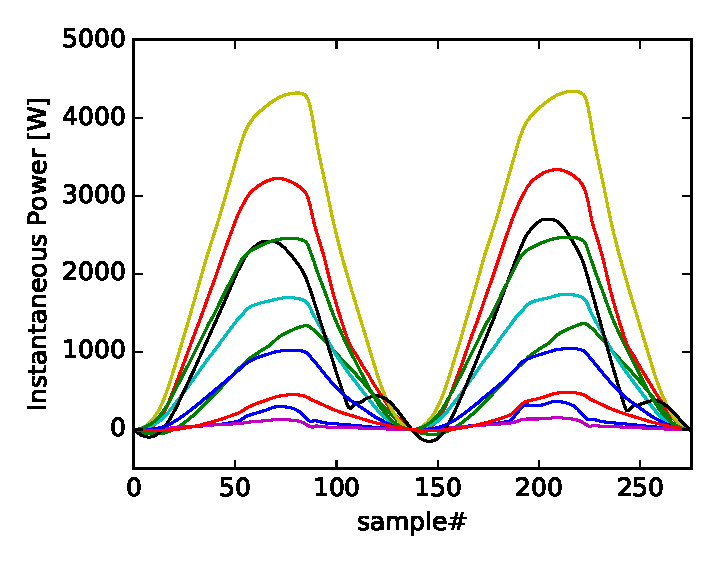
\includegraphics[width=0.45\textwidth]{varbolt/matrixW.pdf}
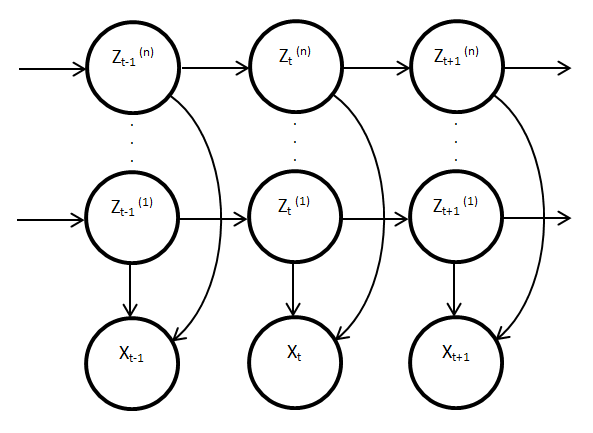
\includegraphics[width=0.45\textwidth]{varbolt/FHMM.png}
  \caption[VarBOLT: Aggregate instantaneous power waveforms and extracted candidate waveforms.]{(a): Matrix $X$ containing aggregate instantaneous power waveforms alongside the aggregate power. (b): Matrix $W$ containing candidate component waveforms. (c): Representation of a Factorial Hidden Markov model}
  \label{figure1_vb}
\end{figure*}

%$\mathfrak{z}_i$
FHMMs are a generalization of Hidden Markov Models in which multiple hidden states evolve independently in parallel~\cite{ghahramani1996factorial}. See Figure \ref{figure1_vb}c for a representation of the associated graphical model. When the parameters of the individual HMM chains are known, energy disaggregation can be posed as the decoding problem for FHMMs. However, obtaining these paramaters is usually prohibitively expensive. On the other hand, unsupervised energy disaggregation can be posed as the learning problem on this graphical model.\\
Because of its factorial nature, the probability of the observation at time $t$, $x_t$, is a function of the joint hidden state $z_t$, with $t \in \{1,...,T\}$. In general, the latent variables of FHMMs are modeled as categorical variables, which could lead to computationally tractable solutions (e.g., \cite{jang2016categorical}). In our case we restrict $z_t$ to be binary, specifically Bernoulli distributed. Assuming binary hidden states removes some of the ambiguity inherent to the learning problem: every latent representation with categorical variables can be decomposed into a representation with binary variables, i.e. by assigning a binary variable for each categorical state. This binary decomposition is unique and in a sense maximal. However, binary decompositions can be aggregated into exponentially-many categorical decompositions, i.e. any combination of binary latent variables can be joined into one categorical variable. In order to avoid this ambiguity, we restrict the latent variables to be binary.\\
Since hidden states are assumed to be binary and multiple hidden states evolve in parallel, $z_t \in Z  = \{0,1\}^C$ with $C$ being the number of parallel hidden chains. Thus, the joint likelihood can be expressed as:
\begin{align}
p(x_{1:T},z_{1:T}) = \prod_t^T p(x_t|z_t)\prod_i^C p(z_{t,i}|z_{t-1,i})p(z_{0,i})
\end{align}

For the application of energy disaggregation, we choose a representation of the aggregate observation similar to our prior work~\cite{lange2016bolt}, i.e. the observation $x_t$ constitutes the aggregate instantaneous power waveform aligned by zero-crossings detected in the voltage line, thus $x_t \in \mathbb{R}^N$ with $N$ being the number of samples per voltage cycle. Figure \ref{figure1_vb}a shows aggregate instantaneous power waveforms alongside the observed aggregate active power over time. Since instantaneous power is additive, we model $p(x_t|z_t)$ to be a Gaussian distribution with $p(x_t|z_t) = \mathcal{N}(x_t | Wz_t, \alpha I)$ where $\alpha$ is a variance parameter, $W \in \mathbb{R}^{N \times C}$ is a matrix containing the power waveforms of the inferred components and is not assumed to be known. Figure \ref{figure1_vb}b shows an example of inferred power waveforms.\\
Baum-Welch, an Expectaction-Maximization algorithm, is a prominent algorithm for the learning problem in Hidden Markov Models. Baum-Welch makes model updates based on the expected time spent in states, the expected number of state transitions and the expected number of times a state emits an observation. An efficient algorithm to compute these quantities is the forward-backward algorithm. The forward-probabilities (\ref{eq:forward_probs}) can be computed recursively. Given the forward probabilities, the filtering distribution can be computed according to (\ref{eq:filt_rec}).
%\begin{equation}
\begin{align}
p(x_{1:t},z_t) &= p(x_t|z_t) \sum_{z' \in Z} p(z_t|z') p(z_{t-1}, x_{1:t-1}) \label{eq:forward_probs}\\
p(z_t|x_{1:t}) &= \frac{p(x_{1:t},z_t)}{\sum_{z' \in Z} p(x_{1:t},z')} \label{eq:filt_rec}
\end{align}
%\end{equation}
Because the number of possible latent states $z$ grows exponentially with the number of components, evaluating (\ref{eq:forward_probs}) is intractable for FHMMs. However, as we will show later, ideas from Variational Inference can be used to approximate forward-probabilities.\\
 Variational Inference is a tool to deal with intractable posterior distributions and relies on an auxiliary or variational distribution $Q$ governed by the variational parameter $\Theta$. Posterior inference in $Q$ is required to be tractable, which is usually achieved by making independence assumptions. To paraphrase the main idea behind Variational Inference: in order to perform inference on a distribution $P$ with intractable posterior, variational parameters $\Theta$ are chosen in such a way that $Q$ best approximates $P$ and then inference is performed on $Q$ instead of $P$. For our application, $P$ is the filtering distribution, i.e. (\ref{eq:filt_rec}), and we choose $Q$ to be an independent multivariate Bernoulli distribution with density $q_\sigma(z_t) = \prod_i^C \sigma_i^{z_{t,i}}(1-\sigma_i)^{1-z_{t,i}}$ and with $\sigma_i$ being the coin-flip probabilities of the latent variables. For the conditional $q_\sigma(z_t|x_t)$, we assume the coin-flip probabilities to be functions of the conditioning variable $x_t$, i.e. $q_\sigma(z_{t} =\vec{1}|x_t) = \sigma_{t} = f_\Theta(x_t)$. Because we want $Q$ to capture the temporal dependencies present in $P$, we chose $f$ to be a recurrent deep neural network governed by the variational parameters $\Theta$ (which in this case constitute the weights of the neural network). This in turn means that $\sigma_t = f_\Theta(x_{1:t})$ is a function of all previous observations $x_{1:t}$, i.e. $Q$ is also a filtering distribution: $q(z_t|x_{1:t})$. Note that this implies that the auxiliary distribution does not assume temporal independence between latent variables but assumes independence between elements of the latent variable at any given time.\\
The evidence lower bound (ELBO) as a variational objective can be derived as follows~\cite{blei2011variational}:
\begin{align}
\mathcal{L} &= \log p(x_{1:t}) - D_{KL}(q(z_{t}|x_{1:t}) || p(z_{t}|x_{1:t})) \label{eq:lower_bound}\\
&=  \mathbb{E}_{Q}[\log p(x_{1:t},z_{t})] - \mathbb{E}_{Q}[\log q(z_{t})] \label{eq:elbo_vb}
\end{align}
Note that because of the equivalence of (\ref{eq:lower_bound}) and (\ref{eq:elbo_vb}), maximizing (\ref{eq:elbo_vb}) is equivalent to maximizing (\ref{eq:lower_bound}). This means that optimizing the parameters of $P$ and $Q$ with respect to to (\ref{eq:elbo_vb}) leads to maximization of the log-likelihood of the data as well as minimization of the posterior divergence. Although the second expectation of (\ref{eq:elbo_vb}) usually has an analytical solution, evaluating the first expectation is usually achieved by sampling from $Q$~\cite{ranganath2014black}. However, approximating the expression by sampling disconnects the optimization problem from the variational parameters $\Theta$, i.e. $Q$ vanishes from the optimization problem. For some continuous non-conjugate distributions, this problem can be avoided by the re-parameterization trick~\cite{ruiz2016generalized}, i.e. by finding a deterministic and differentiable function that provides samples of $Q$ given the variational parameters $\Theta$ and some random noise. For binary non-conjugate distributions such as the Bernoulli such a function does not seem to exist~\cite{kingma2013auto}.\\
We circumvent this problem by approximating the true filtering distribution, i.e. estimate $\hat{p}(z_{t}|x_{1:t})$ with the help of $Q$. Given estimates $\hat{p}(z_{t}|x_{1:t})$, the $\sigma^*$ as a function of $\Theta$ resulting in the lowest forward KL-divergence can be obtained, i.e. $\sigma^* = \arg \min_{\sigma}\sum_t D_{KL}(\hat{p}(z_{t}|x_{1:t}) || q_\sigma(z_{t}|x_{1:t}))$. Given $\sigma^*$, the binary cross-entropy loss between $\sigma$ and $\sigma^*$ ($H(\sigma_t, \sigma_t^*)$) is then minimized in order to minimize the forward KL-divergence of the posterior.\\
Minimizing the binary cross-entropy loss between $\sigma$ and $\sigma^*$ minimizes the posterior divergence but since the parameters of $P$ (the component waveforms $W$) are not known, the model needs to be forced to explain the aggregate signal explicitly. Otherwise the free parameter $W$ will be abused to minimize the divergence without explaining the data. Thus, we additionally maximize $\mathbb{E}_{Q}[\log \hat{p}(z_t, x_{1:t})]$ in order to explain the aggregate waveforms. Hence, the objective function becomes:
\begin{align*}
L(\sigma, W) &=  \sum_t\mathbb{E}_Q[\hat{p}(z_t, x_{1:t})] - H(\sigma_t, \sigma_t^*)\\
\text{with:\ \ } \sigma_t^* &= \min_{\sigma}D_{KL}(\hat{p}(z_{t}|x_{1:t}) || q(z_{t}|x_{1:t})) \\
 &= \mathbb{E}_{\hat{p}(z_{t}|x_{1:t})}[z] \\
\text{and:\ \ } -H(\sigma_t, \sigma_t^*) &= \sigma_t^*\log(\sigma_t) + (1-\sigma_t^*)\log(1-\sigma_t) \\
\end{align*}
To sum up the main ideas of this paper:
\begin{itemize}
\item Computing the filtering recursion required for the E-step of Baum-Welch is prohibitively expensive since it requires a summation over exponentially-many latent configurations.
\item An auxiliary distribution $q(z_t|x_{1:t})$ that assumes independence between elements in $z_t$ is introduced, which allows for approximating $\hat{p}(z_t|x_{1:t})$. Note that $q$ does not assume independence over time steps. The independence structure of the auxiliary distribution is then exploited to approximate the filtering recursion efficiently circumventing summation of exponentially-many latent configurations.
\item In order to optimize the parameters of the auxiliary distribution, the variational parameters minimizing the KL-divergence between $P$ and $Q$, i.e. $\sigma^*$, are estimated and the binary cross-entropy loss between the predicted parameters $\sigma$ and the optimal $\sigma^*$ is minimized. As we will show later, this is equivalent to minimizing the KL-divergence but circumvents the re-parameterization trick and allows for a compact representation of the problem.
\end{itemize}
Note that we interchangeably call $\sigma$ and $\Theta$ variational parameters. However, in reality, $\sigma$ is a function of the true variational parameters, i.e. the neural network weights $\Theta$, and when a loss is defined with respect to $\sigma$ then gradients with respect to $\Theta$ can be obtained by application of the chain rule.\\
In the next section, we will discuss how to obtain estimates of the filtering distribution probabilities, i.e. $\hat{p}(z_t|x_{1:t})$.

\section{Estimating filter distribution probabilities}
\label{sec:esti}
When using the forward-algorithm to obtain the filtering distribution $p(z_{t}|x_{1:t})$ for FHMMs, the computational complexity is in $\mathcal{O}(2^{2C}T')$ with $C$ being the number of components and $T'$ being the number of discrete time steps. In this work, we propose a learning algorithm that operates in $\mathcal{O}(C^{\epsilon+1}T)$ with $C^\epsilon$ being the number of candidate latent state configurations being considered and $T \ll T'$ (by reducing decision variables) and $\epsilon < C$ (by enforcing sparsity).
\subsection{Reducing decision variables}
For the problem of energy disaggregation, the aggregate observation is highly non-iid, i.e. instantaneous power waveforms tend to repeat themselves over time since they are associated with the operational state of appliances (and these do not change very often). This implies that, as long as the aggregate observations have not changed significantly, the latent states will not have changed and no new decision needs to be made. Thus, by employing a simple change-point detector that extracts points in time, also called events, where a significant change in the aggregate power was observed, the number of decision variables can be reduced significantly. Let the number of detected events be $T$. Reducing the number of decision variables reduces the complexity to $\mathcal{O}(2^{2C}T)$. Depending on the change point detector, $T$ is often three orders of magnitudes smaller than $T'$~\cite{wild2015new}.

\subsection{Enforcing sparsity}
A portion of the latent space can be excluded by enforcing sparsity of the latent variables. Usually only a small number of appliances are active at any given time. Thus latent configurations where more than $\epsilon$ components are active can be excluded. Let $\mathcal{Z} = \{z \in \{0,1\}^C|\sum_i z_i < \epsilon \}$ be the set of sparse candidate latent configurations. We assume that $p(x_{1:t}, z_t = z_i) = 0$ for all $z_i \notin \mathcal{Z}$. This assumption allows us to evaluate $p(z_t|x_{1:t})$, since the denominator of equation (\ref{eq:filt_rec}) has become tractable. This assumption reduces the complexity to $\mathcal{O}(C^{2\epsilon}T)$ with $|\mathcal{Z}| \in \mathcal{O}(C^{\epsilon})$.

\subsection{Variational approximation of $p(z_t|x_{1:t})$}
For many problems modeled with FHMMs, such as energy disaggregation, $p(z_t|x_t)$ and therefore $p(z_t|x_{1:t})$ are highly multi-modal distributions. However, since the auxiliary conditional distribution $Q$ assumes independence between elements of $z$, $Q$ is unable to learn the multi-modality of $p(z|x)$. However, $Q$ is able to either learn $\arg \max_z p(z|x)$ or $\mathbb{E}_{p(z|x)}[z]$. These two modeling choices are reflected in either minimizing the forward $D_{KL}(P||Q)$ or reverse $D_{KL}(Q||P)$, respectively. It can be shown that:
\begin{align*}
 \arg \min_{\sigma} D_{KL}(P||Q_\sigma) &= \mathbb{E}_{p(z|x)}[z] \\
 \arg \min_{\sigma} D_{KL}(Q_\sigma||P) &= \arg \max_z p(z|x)
 \end{align*}
Viterbi learning was proposed as a faster alternative to Baum-Welch. For Viterbi learning the model parameters are updated based on the most probable path $z^*_{1:T} = \arg \max_{z_{1:T}} p(z_{1:T} | x_{1:T})$.\\ Since minimizing the reverse KL-divergence forces $Q$ to learn the most probable mode of $P$, minimizing the reverse KL-divergence approximates Viterbi learning but tends to underfit considerably. On the other hand, minimizing the forward KL-divergence seems to preserve more information about state posterior probabilities. However, as we will show later, our proposed method does not correspond fully to learning like Baum-Welch, i.e. updating the model based on $p(z_t|x_{1:\boldsymbol{T}})$, but rather updating based on $p(z_t|x_{1:\boldsymbol{t}})$, that is, making model updates based on forward-probabilities alone whilst ignoring backward-probabilities.\\
As discussed earlier, the Baum-Welch algorithm as well as Viterbi learning require computations that are quadratic in the numbers of hidden states. Even with the domain-specific sparsity assumptions introduced earlier, computations that are quadratic in the number of latent configurations are still prohibitively expensive. The key insight into circumventing these computations is the fact that the filtering distribution at time $t$, i.e. $p(z_t|x_{1:t})$ can be approximated by exploiting the independence structure of $Q$, i.e. the fact that the auxiliary distribution assumes independence between components at any single point in time. Starting with equation (\ref{eq:forward_probs}):
\begin{align*}
&p(x_{1:t},z_t) \\
&= p(x_t|z_t) \sum_{z' \in \mathcal{Z}} p(z_t|z') p(z_{t-1} = z', x_{1:t-1})\\
			&\approx p(x_t|z_t) \sum_{z' \in \mathcal{Z}} p(z_t|z') \boldsymbol{q}(z_{t-1} = z'|x_{1:t-1})p(x_{1:t-1})\\
			&= p(x_t|z_t) \sum_{z' \in \mathcal{Z}} p(z_t|z') \prod_i \sigma_{t-1,i}^{z'_i} (1-\sigma_{t-1,i})^{1-z'_i}p(x_{1:t-1})
\end{align*}
Note that FHMMs components switch independently, i.e. $p(z|z') = \prod_i p(z_i | z'_i)$ and let $\pi(m,n)$ be the state-transition probabilities. Because $q(z_{t}|x_{1:t})$ assumes independence between elements of $z_{t}$, we can simplify the expression by recursively pulling out elements of $q(z_{t}|x_{1:t})$, ultimately allowing us to rewrite a sum over all possible $z$ into a sum over the number of components, i.e. circumventing computations that grow exponential with the number of parallel latent states:
\begin{align*}
p(x_{1:t},z_t)&\approx p(x_t| z_t)p(x_{1:t-1})\sum_{z' \in Z} \prod_i p(z_{t,i} = z_i | z_{t-1,i} = z'_i) \sigma_{t-1,i}^{z'_i} (1-\sigma_{t-1,i})^{1-z'_i}\\
&=p(x_t|z_t)p(x_{1:t-1})\sum_{z' \in Z} \prod_i (z_i \pi(1 , z'_i) + (1-z_i) \pi(0 ,z'_i))\sigma_{t-1,i}^{z'_i} (1-\sigma_{t-1,i})^{1-z'_i} \\
&= p(x_t|z_t)p(x_{1:t-1})\sum_{i}z_i\sigma_{t-1,i} \pi(1 , 1)+ z_i (1- \sigma_{t-1,i}) \pi(1 , 0) \\
  &\text{\ \ \ \ \ \ \ \ \ \ \ \ \ \ \ }\text{\vspace{1in}}  +(1-z_i) \sigma_{t-1,i} \pi(0, 1) + (1-z_i)(1- \sigma_{t-1,i}) \pi(0, 0)\\
&= \hat{p}(x_{1:t}, z_t)
\end{align*}
This allows us to approximate the forward probabilities $p(z_t, x_{1:t})$ based on $\sigma_{t-1}$ as provided by $Q$ and $W$ as a parameter of $P$. Since we can compute $\hat{p}(z_t, x_{1:t})$ for all sparse $z \in \mathcal{Z}$, we can approximate the filtering distribution $\hat{p}(z_t | x_{1:t})$ according to equation (\ref{eq:filt_rec}). Note that, since we are only interested in the filtering distribution, $p(x_{1:t-1})$ does not need to be modeled because it cancels out.\\ Let $\sigma^* = \mathbb{E}_{\hat{p}(z_t = z | x_{1:t})}[z]$. Even though $\sigma^*$ is a function of $W$, we treat $\sigma^*$ as a constant and do not allow the gradient of $W$ to flow into $\sigma^*$. This avoids $W$ being exploited to minimize the posterior divergence instead of explaining the aggregate data. Note that, when allowing the gradient of $W$ to flow into $\sigma^*$, the algorithm will infer nonsensical component waveforms, i.e. waveforms that draw significant power when the voltage is $0$. Based on the same reasoning, we do not allow the gradient of $\sigma$ to flow into $\mathbb{E}_Q[\hat{p}(z_t, x_{1:t})]$.\\
Thus by exploiting the independence assumption of the auxiliary distribution, the computational complexity estimating the filtering distribution can be reduced to $\mathcal{O}(C^{\epsilon+1} T)$.\\
There is at least one example in the literature showing an application of variational inference for learning in FHMMs: in \cite{ng2016scaling} Gaussian copulas are paired with variational inference to minimize an objective including the reverse KL-divergence, thus circumventing the problem of having to approximate the filtering distribution. Furthermore, although not applied to sequential data and therefore not modeling temporal dependencies between latent variables, previous work has proposed approaches for the subproblem of estimating the gradient through binary stochastic units, e.g. \cite{raiko2014techniques,bengio2013estimating}. When temporal dependencies are removed, authors in ~\cite{tang2013learning} arrive at a similar solution to ours. Their respective loss is derived as: $L_{T\&S} = \sum_m \overline{w}^{(m)}[\log p(x|z^{(m)}) + \log p_{\sigma}(z^{(m)}|x)]$ with $\overline{w}^{(m)}$ being normalized importance weights of configuration $z^{(m)}$. Note that, if the sparsity constraints introduced here were to be applied, the importance weights would approximate $p(z|x)$. Also note that in that case, even though motivated differently, the gradient updates with respect to the component activation probabilities $\sigma$ are equivalent when temporal dependencies are not modeled. This justifies the seemingly arbitrary choice of minimizing the cross-entropy loss, i.e. $H(\sigma, \sigma^*)$ (instead of e.g. ($\sigma - \sigma^*)^2$). 

It can be shown that:
\begin{align*}
\frac{\partial L_{T\&S}}{\partial \sigma_i}=& \frac{1}{-(1-\sigma_i)}[1-\sigma_i^*]+ \frac{1}{\sigma_1}[\sigma_i^*]\\
 =&  \frac{\partial (1-\sigma_i^*)\log(1-\sigma_i) + \sigma_i^*\log(\sigma_i)}{\partial \sigma_i} \\
 =&  \frac{\partial H(\sigma, \sigma^*)}{\partial \sigma_i} 
\end{align*}

\section{Modeling temporal dependencies}
Building on experience from previous work~\cite{lange2016bolt}, the main objective of modeling the temporal dependencies between latent states is temporal regularization. Specifically for the problem of energy disaggregation, this means that when a single appliance changes its state, only one and not multiple components change state. Without modeling the temporal dependencies, models tend to `stitch', i.e. when a single appliance turns on, multiple model components switch states. Also without modeling temporal dependencies, the model `recycles' components, e.g. appliance $a$ might be explained by components $1$ and $2$, then appliance $b$ is explained by components $2$ and $3$ and appliance $c$ is explained by components $1$ and $3$. A linear mapping from components to appliances then becomes impossible.\\
Furthermore, for energy disaggregation, introducing fixed state transition probabilities is problematic because of vast differences in the power consumption of appliances. When every component pays a fixed cost for switching ($\pi(0,1)$ or $\pi(1,0)$), appliances with a high power consumption can still afford to be explained by multiple components because the cost for under-estimating the aggregate is higher than multiple switching costs. At the same time, appliances that consume little power will be ignored, since when they turn on, the associated increase in aggregate loss does not outweigh the switching cost.\\
To overcome this problem, we additionally model the difference signal $\delta x_t = x_t - x_{t-1}$ similar to ~\cite{kolter2012fhmm}. Note that although technically the graphical model changes (see Figure \ref{graph_mod}), $\pi$ can also be viewed as a function of $\delta x_t$, i.e. the switching probabilities depend on how well each component explains $\delta x_t$. We define switching probabilities associated with each component turning \emph{on} or \emph{off} at time $t$. Additionally, we define a switching probability associated with no component switching.

\begin{figure}
\centering
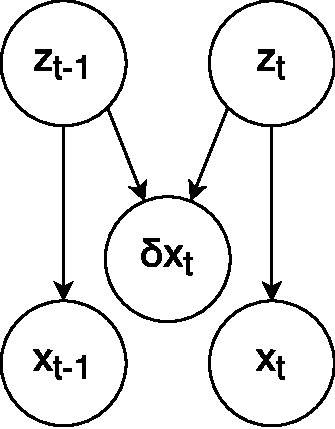
\includegraphics[width=0.35\linewidth]{varbolt/gmod.pdf}
\caption[VarBOLT: Graphical Model when additionally modeling the difference signal.]{\label{graph_mod} Graphical Model when additionally modeling the difference signal $\delta x_t$}
\end{figure}
Let,
\begin{align*}
\mathcal{I}(t,i) &= exp[-\beta||W_{i:} - \delta x_t||] & \text{\ \ \ \ \ \ (on-switch)}\\
\mathcal{O}(t,i) &= exp[-\beta||W_{i:} + \delta x_t||]&\text{\ \ \ \ \ \ (off-switch)}\\
\mathcal{X}(t) &= exp[-\beta||\delta x_t||]& \text{\ \ \ \ \ \ (no-switch)}
\end{align*}

Following the intuition gained earlier, we estimate the filtering distribution as,

\begin{equation}
\begin{aligned}
\hat{p}(z_t = z, x_{1:t}) = p(x_t|z_t = z)p(x_{1:t-1})
[&\sum_i^C (\sigma_{t-1,i}(1-z_i)\mathcal{O}(t,i) + (1-\sigma_{t-1,i})z_i \mathcal{I}(t,i)) \\
+ &\prod_i^C(z_i\sigma_{t-1,i} + (1-z_i)(1-\sigma_{t-1,i})) \mathcal{X}(t)] \label{eq:final_model}
\end{aligned}
\end{equation}%Note that forcing each switching component to individually explain $\delta x_t$ and additionally modeling the aggregate $p(x_t|z_t)$ imposes the one-at-a-time constraint implicitly: when two components switch and they both explain the difference, the aggregate power will overshoot by a factor of 2. However, if two components switch that jointly explain the aggregate, then the difference signal will undershoot by half. That means that all cases where multiple components switch incur either big errors in the difference or in the aggregate signal.\\
Note that the model described in equation (\ref{eq:final_model}) models dependencies between components to some degree. The product in the last line can be expanded into all combinations of component configurations where no component switches from $t-1$ to $t$. This factorization allows for a compact and differentiable representation of `no component'-switches without having to enumerate an exponential number of configurations, therefore modeling limited dependencies between components efficiently.

\section{Resulting Algorithm: Variational BOLT}

The resulting algorithm, which we call Variational BOLT, operates in temporal mini-batches of a fixed time-horizon $h$, i.e. the data is sequentially fed into the neural network and model parameters $\Theta$ and $W$ are updated before a new mini-batch of data is processed. This process is repeated until convergence. Algorithm 1 explains the process in pseudo-code.


\begin{algorithm}[htb]
\SetKwInOut{Input}{input}\SetKwInOut{Output}{output}
\Input{Dataset $X$ of size $T \times N$}
\Output{Trained model parameters $W$ and $\Theta$}
Initialize $W$ by clustering and $\Theta$ randomly\;
\While{not converged}{
	$t \leftarrow 0$\;
	$\sigma_0 \leftarrow \vec{0}$\;
	\While{$t < T$}{
		\For{$t' \in t:t+h$}{
			\emph{Neural Network forward pass}\;
			$\sigma_{t'} = f_\Theta(X[1:t',:])$\;
			\For{$z \in \mathcal{Z}$}{
				Compute $\hat{p}(x_{1:t'}, z)$ based on (\ref{eq:final_model})\;
			}
			\For{$z \in \mathcal{Z}$}{
				Compute $\hat{p}(z| x_{1:t'})$ based on (\ref{eq:filt_rec})\;
			}
			$\sigma^*_{t'} \leftarrow \mathbb{E}_{\hat{p}(z|x_{1:t'})}[z]$\;
		}
		Maximize $\sum_{t' = t}^{t+h}H(\sigma_{t'}, \sigma^*_{t'})$ with respect to $\Theta$\;
		Maximize $\sum_{t' = t}^{t+h}\mathbb{E}_Q[\hat{p}(z, x_{1:t'})]$ with respect to $W$\;
		$t \leftarrow t + h$\;
	}
}
\caption{Variational BOLT in pseudo-code}
\end{algorithm}


The resulting algorithm has similarities to Variational Autoencoders (VAE) as well as Expectation Maximization, specifically the Baum-Welch algorithm. Like VAE, an efficient auxiliary recognition distribution is trained to predict the parameters of the latent distribution. However, the auxiliary distribution is solely used to speed up computations of the filtering recursion. Unlike VAE and like EM, instead of approximating intractable expectations by sampling latent states from the recognition distribution, updates are computed based on a fixed set of possible hidden states.

\section{Experiments}
\begin{figure}
\centering
%\vspace{0pt}
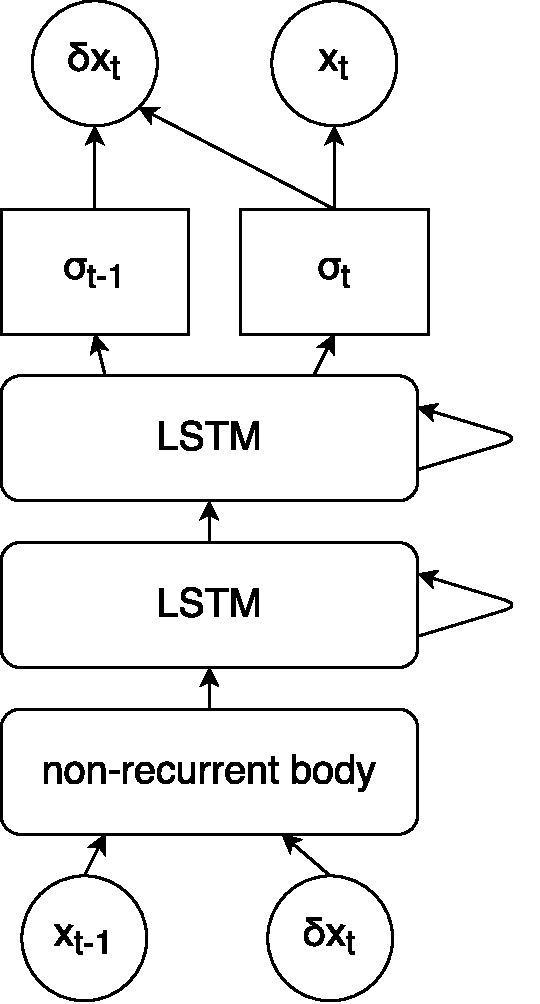
\includegraphics[width=0.35\linewidth]{varbolt/lstm_topo.pdf}
\caption[VarBOLT: Neural Network Topology]{\label{topo} Topology of the neural network}
%\vspace{10pt} 
\end{figure}
%\end{minipage}
%\vspace{0pt} 

%\begin{minipage}{0.50\textwidth}
Experiments were conducted on the publicly-available REDD~\cite{kolter2011redd} dataset. The dataset contains current and voltage readings at the main distribution panel with a sampling rate of 16kHz and breaker level power readings with a sampling frequency of 0.3Hz. The neural network used to predict $q(z_t = \vec{1}|x_{1:t})$ is a 4 layer recurrent neural network. The bottom two layers constitute non-recurrent $tanh$ layers with 200 output units each. The top two layers are LSTM-layers with $sigmoid$-activations each with 100 and 10 output units respectively. This means that 10 components were extracted and maximally 6 out of these 10 inferred components were allowed to be active at any given time ($\epsilon = 6$). Figure \ref{topo} shows a graphical depiction of the neural network.\\
Change points of the aggregate power were detected by an event detection algorithm: Let $p(t)$ be the aggregate power at time $t$. The maximum value of the absolute difference in the power signal within a window of 5 time steps was extracted. Every window then casts a vote for the highest absolute power difference. However, only these timestamps for which $|p(t) - p(t-1)| > 50W$ holds can receive a vote. Every time stamp that received more than 3 votes is considered an event. Then, in order to reduce the number of decision variables, the mean instantaneous power waveforms in between events was extracted, and these constitute the set of $T$ values of $x_t$.\\
The neural network was then fed $x_t$ and $\delta x_t = x_t - x_{t-1}$ and tasked to explain $x_{t+1}$ and $\delta x_t$. In order to speed up convergence, the appliance waveforms $W$ were initialized by the cluster centroids obtained by applying K-Means to the difference signal $\delta x_t$. In the experiments the hyper-parameters $\alpha$ and $\beta$, i.e. the variance of the difference and aggregate model were kept at $1$.\footnote{Exploring the hyperparameter space as well as experimenting with different $W$ initializations and emission probability models could be a promising future research endeavor.} The model was trained for 200 iterations. For inference, the filtering distribution probabilities were simply binarized: $z = \sigma > 0.5$.

%\end{minipage}
%\begin{minipage}{0.45\textwidth}


\subsection{Results}

\begin{table}
%\small
\centering
\begin{tabular}{lll}
 (a)    & AFAMAP     & VarBOLT \\
   Circuit                 &  (supervised*)& (unsupervised) \\
                        \hline
                        \hline
    Microwave & 97.5\% / 66.1\%  & 88.8\% / 8.0\%     \\
    Bath GFI    & 82.7\% / 70.8\% & 71.9\% / 40.2\%      \\
    Electronics     & 41.6\% / 0.8\%    & 87.8\% / 40.7\%  \\
    Kitch. Out. 1 & 37.5\% / 12.9\%       &\ 8.6\% / 32.8\%  \\
    Furnace & 91.7\% / 70.8\%  & 85.0\% / 50.6\%  \\
    Kitch. Out. 2 .& 45.2\% / 16.0\%       & \ 5.3\% / 70.1\%  \\
     Washer/Dryer & 98.8\% / 73.6\%   & 97.3\% / 72.3\% \\
     \hline
     \vspace{0.01cm}\\
      (b)& NFHMM     & VarBOLT \\
      &  (unsupervised)& (unsupervised) \\
      \hline
      \hline
      Overall panel & 0.25 & 0.63 \\
      \hline
  \end{tabular}
  \caption[VarBOLT: Performance comparison]{(a) Performance comparison to AFAMAP, a supervised inference technique paired with an unsupervised strategy of obtaining ground truth. Performance is measured in Precision / Recall. (b) Performance comparison with NFHMM, another end-to-end unsupervised approach, in GSPA.}
  \label{vbolt:results}
  \end{table}

\begin{figure}[!h]
\centering
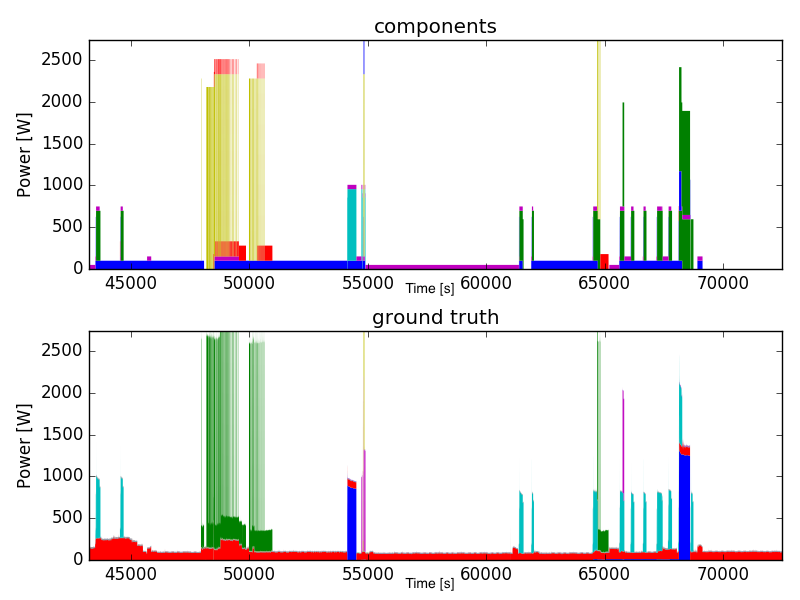
\includegraphics[width=0.8\linewidth]{varbolt/aggregate.png}\\
\rule{0.5\linewidth}{0.4pt}
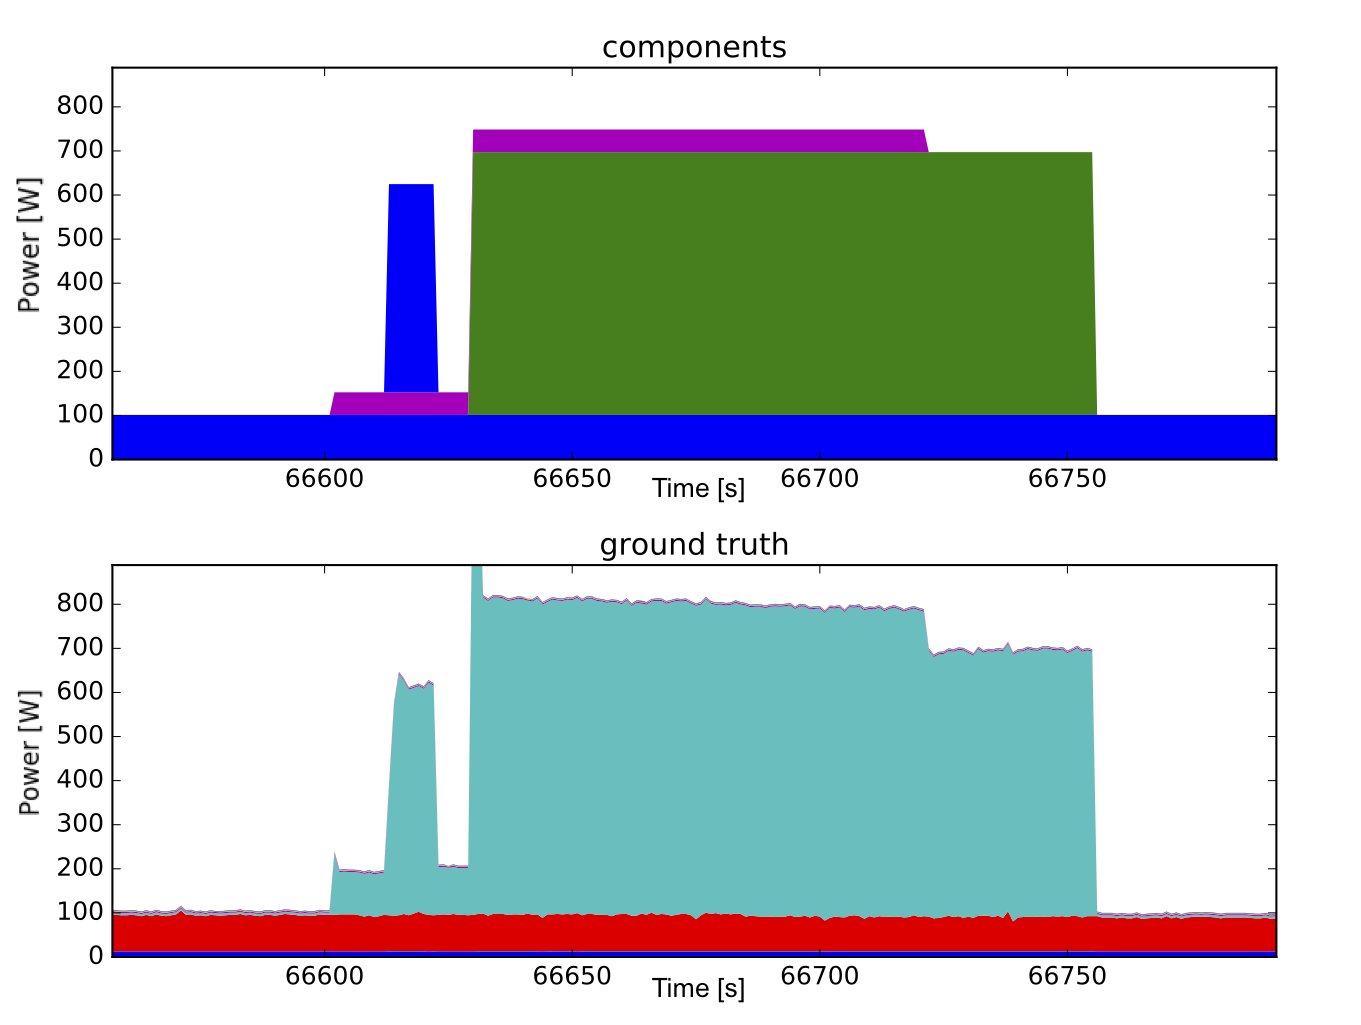
\includegraphics[width=0.8\linewidth]{varbolt/furnace.png}
\caption[VarBOLT: Disaggregation performance and an example of `over-disaggregation'.]{\label{furnace} Top: Inferred components as well as circuit level ground truth. Bottom: An example of `over-disaggregation' of the furnace.}
\end{figure}

Since appliances were sub-metered at the circuit level and some circuits contain multiple appliances, precision and recall are used as a metric. ``Recall measures what portion of a given circuit’s energy is correctly classified, while precision measures, of the energy assigned to a circuit, how much truly belonged to that circuit''~\cite{kolter2012fhmm}. For every pair of inferred component and circuit, precision and recall were computed and the component resulting in the highest $(prec + recall)/2$ was selected for this circuit.\\
Note that because we assume $z$ to be binary, we implicitly assume appliances to be 2-state, i.e. they can either be \emph{on} or \emph{off}. However, appliances like e.g. a furnace are composed of multiple sub-elements. In that case, the proposed model `over-disaggregates', i.e. it assigns a component for every sub-element. An example of `over-disaggregation' can be seen in Figure \ref{furnace}. Furthermore, some appliances have different power levels according to their operational state, i.e. a hair-dryer has different heat settings. In this case, the proposed methods assigns different components for the same appliances. Note that supervised inference techniques usually do not suffer from these problems. This is why we expect supervised inference algorithms to outperform our approach. Table \ref{vbolt:results}(a) shows a comparison with AFAMAP~\cite{kolter2012fhmm}. AFAMAP is a supervised inference algorithm paired with an unsupervised strategy of obtaining model parameters for the individual HMM chains.
We also compare the performance to a fully unsupervised method based on Non-parametric FHMMs (NFHMM) proposed in \cite{jia2015fully} (\ref{vbolt:results}(b)). As a performance criterion, they propose GSPA (worst 0 - 1 best). GSPA does not measure differences in power but rather differences between activations, i.e. circuit power traces are binarized and then GSPA measures a weighted ratio between the intersection and union between binarized ground thruth and estimates.


\section{Conclusion \& Future Work}
We proposed a variational learning algorithm for discrete Factorial Hidden Markov Models and applied it to the problem of energy disaggregation. The algorithm compares promisingly to a supervised inference algorithm that is paired with an unsupervised approach of obtaining ground truth. When compared to another end-to-end unsupervised approach, our proposed method significantly outperforms it. An implementation in \emph{keras}~\cite{chollet2015} can be found at: \emph{\url{https://github.com/INFERLab/varbolt}}. Once the auxiliary distribution is trained, the corresponding neural network could in principle be deployed to sensing hardware located at the electrical panel for on-premise real-time inference.\\
Furthermore, we believe that our proposed method opens many interesting research paths as there is still much room for improvement. A possible research path is to combine our methods with ideas from~\cite{tang2013learning}. By sampling candidate hidden configurations, the sparsity constrains made in section 3 can, in principle, be relaxed. This may allow the model to scale up to more components while keeping computational cost low. Furthermore, the current model for the difference signal uses the Euclidean distance to judge the similarity between component waveforms and the difference signal, so investigating other similarity measures could further refine the model since Euclidean distances might overemphasize differences in power over differences in the shape of the waveform.

